\chapter{Exploratory Analysis}
First part of the analysis is to explore the different attributes in the data in order to detect possible patterns or correlations. The exploratory analysis is also used to get an understanding of data and its behaviour. Hence, this chapter is about visualizing the different attributes focusing on their influence on the heat consumption. As the heat in each house is turned off in the summer period, data is segmented such that the summer period is excluded from the data used for modeling. \\

\noindent To get an overview of the heat consumption for each house, the daily average consumption for each house has been calculated and can be seen as a function of the time in the following figure. 
\begin{figure}[H]
    \centering
    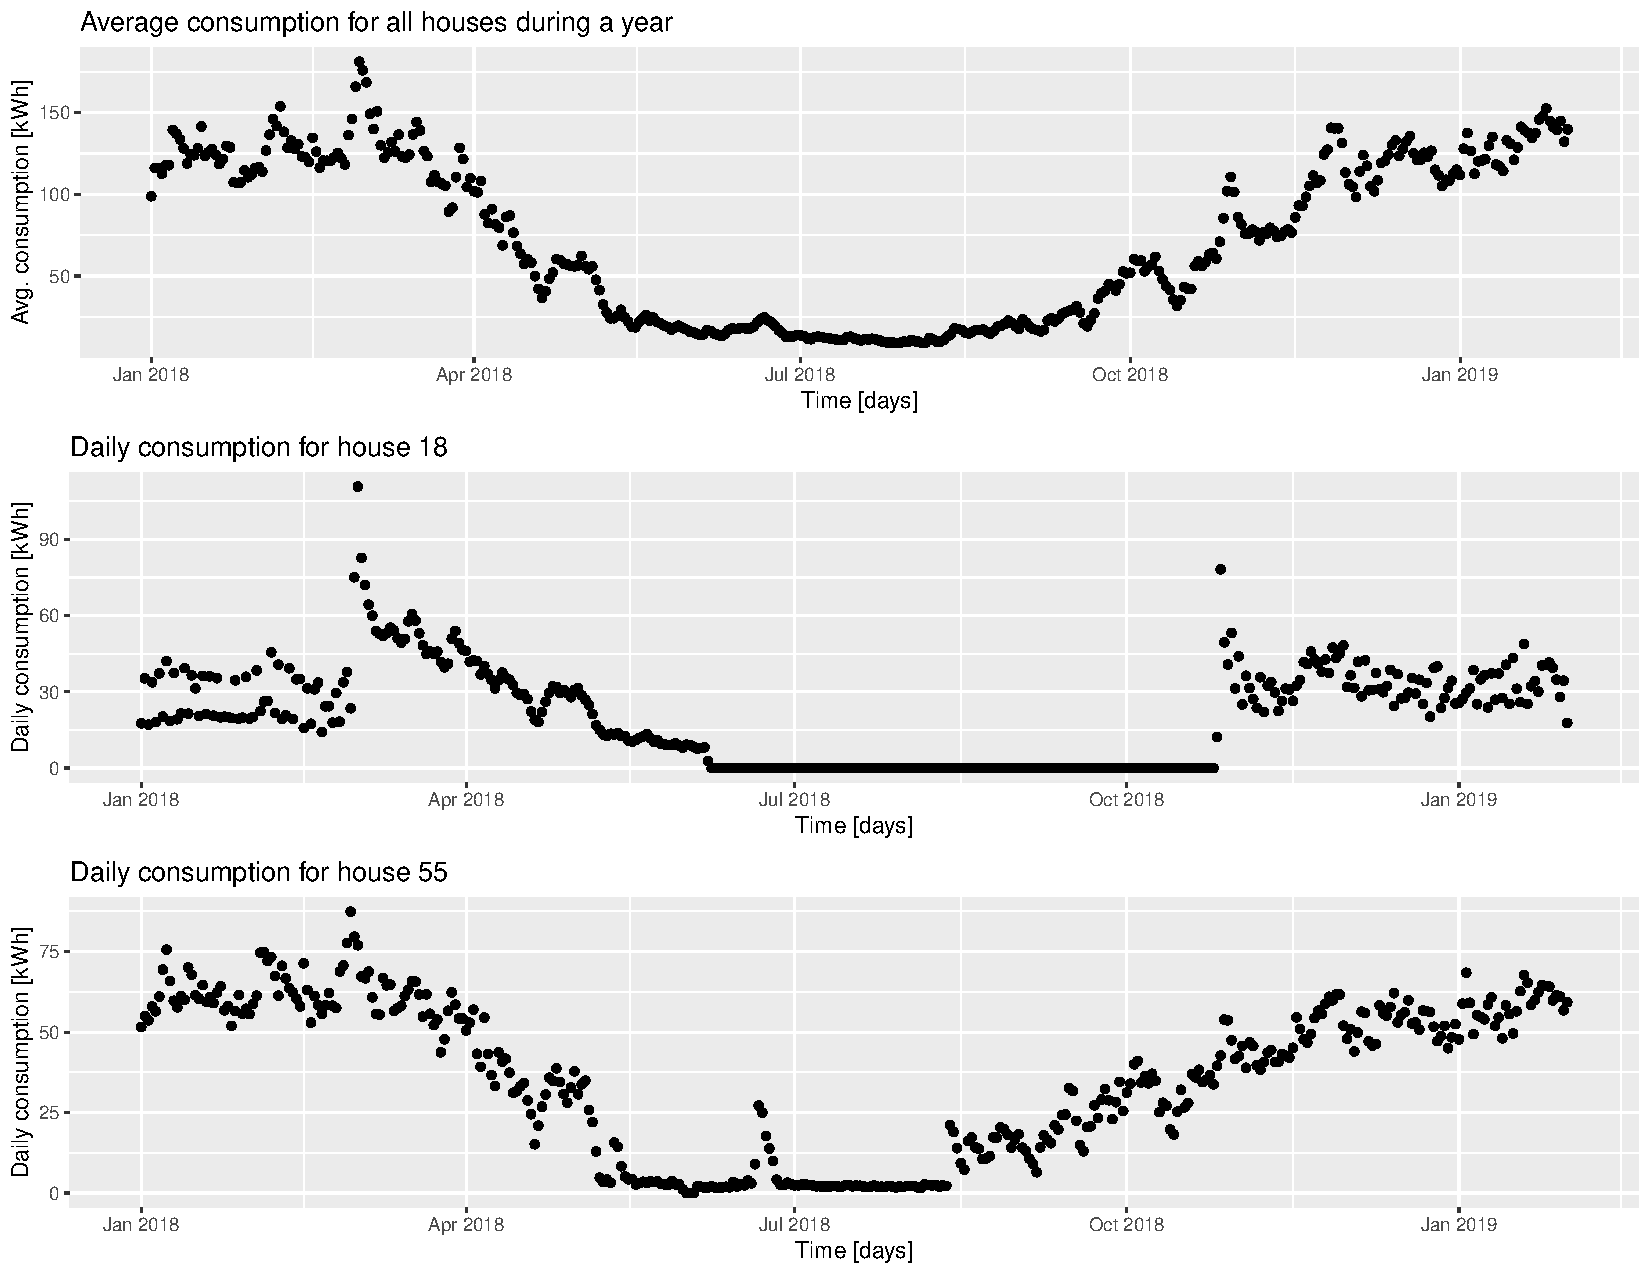
\includegraphics[width=.75\textwidth]{../../../figures/daily_cons.pdf}
    \caption{Daily consumption during a year (2018). The top plot shows the average consumption for all the houses. The plot in the middle shows an example of a house that follows the trend and the last plot shows a house that deviates from the trend}
    \label{fig: daily_cons}
\end{figure}
\noindent Figure \ref{fig: daily_cons} shows the daily average consumption for all the houses and the daily consumption of two houses - one that follows the trend at one that deviates. It can be seen that the slopes around the summer months are close to 0. As mentioned, the data in focus in this project is where the heat is turned on, hence the period where the heat consumption is close to 0 needs to be removed. Exactly how this is done will be explained and discussed in the data segmentation section. All three plots show some unusual high data points around April 2018. This can be due to the fact that is was snowing in Denmark at that time \textcolor{red}{Tilføj reference på det her}. 
\newline \\
\noindent The average of the attributes from the house data is examined through a scatterplot in order to find possible correlations.
\begin{figure}[H]
    \centering
    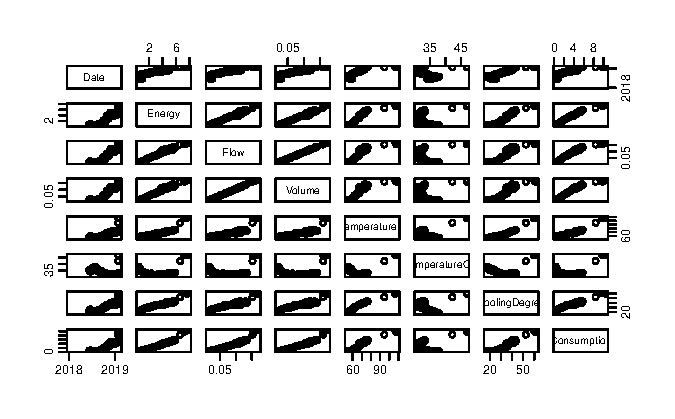
\includegraphics[width=.75\textwidth]{../../../figures/house_attri.pdf}
    \caption{}
    \label{fig: house_attri}
\end{figure}
Figure \ref{fig: house_attri} clearly shows that the consumption is close to 0 in the summer period.  
\textcolor{red}{Pairs af gennemsnitlig house data - vi ser en masse sammenhænge mellem de forskellige attributer. Vi kan se at CoolingDegree skal være over 25, før at varmeforbruget stiger.}
\textcolor{red}{CoolingDegree begynder at stige et stykke tid før flowet stiger, hvilket hænger godt sammen med at når man fx tænder en radiator så stiger CoolingDegree. De efterfølgende radiatorer man tænder øger volumnet.} \\

\begin{figure}[H]
    \centering
    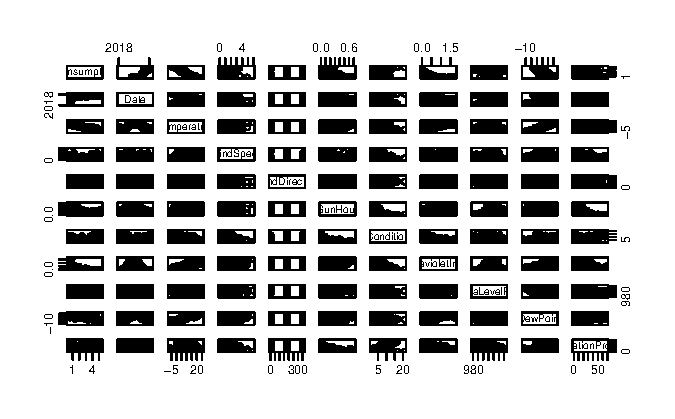
\includegraphics[width=.75\textwidth]{../../../figures/weather_cons_focus.pdf}
    \caption{}
    \label{fig: weather_cons_focus}
\end{figure}

The figure (de udvalgte weather pairs) shows the dependencies between the average consumption of the houses and the weather attributes.
We already know that there is a dependency between the consumption and the time of year. During the summer period there
is almost no consumption. The consumption in this period is probably mostly tap water. The next important thing is the relation
between temperature and consumption. High temperatures tend to imply a higher consumption. And the reason why the consumption
depends so clearly on the time of year can be assumed to that certain periods have similar temperature levels. 
It can also be seen that there is a correlation between dewpoint and consumption. This can be due to the correlation between dewpoint and temperature. \textcolor{red}{Anton nævnte noget med SunHour og Ultravioletindex.}

Figures \ref{fig: house_attri} and \ref{fig: weather_cons_focus} are used to investigate linear relationships which is desired when modeling. If a linear relation is not \textcolor{red}{obtained} this could give rise to a transformation on either the dependent or the independent variable.  

\section{Data segmentation}
When looking at the consumption data, it is useful to distinguish between
periods where the heat is turned off and periods where it is turned on.
The models that will be applied in the following sections should only consider periods with heating turned on, if possible.
Because of the tap-water consumption, this difference is not always clear cut.
The data can be seen as part of two different distributions. One where the
heating is turned off, and one where it is turned on. In this section different 
approaches will be examined on how to distinguish between the two distributions.
The goal is to find some temperature, where it can be assumed that all data points below it
belongs to the distribution with heating turned on. Three approaches will be described below, together with their pros and cons.

\subsection{Segmentation by piece-wise optimization}
The first approach is to make a linear regression on the data with two segments.
A breakpoint $\alpha$ is found, such that the SSE is as small as possible.
The second segment is restricted to being constant. This way the breakpoint
illustrates when the consumption goes from being linearly dependent on the temperature,
to having a constant value. If that assumption holds, all data points below the breakpoint
can be used in the statistical model for analysing heat consumption, and the rest can be discarded
as tap water consumption.

Figure \ref{fig: Consumption-PW} shows the regression for two different houses. On both houses the
line fits rather well with the low-temperature data points. But it is not very accurate around the breakpoint.


\begin{figure}[H]
    \centering
    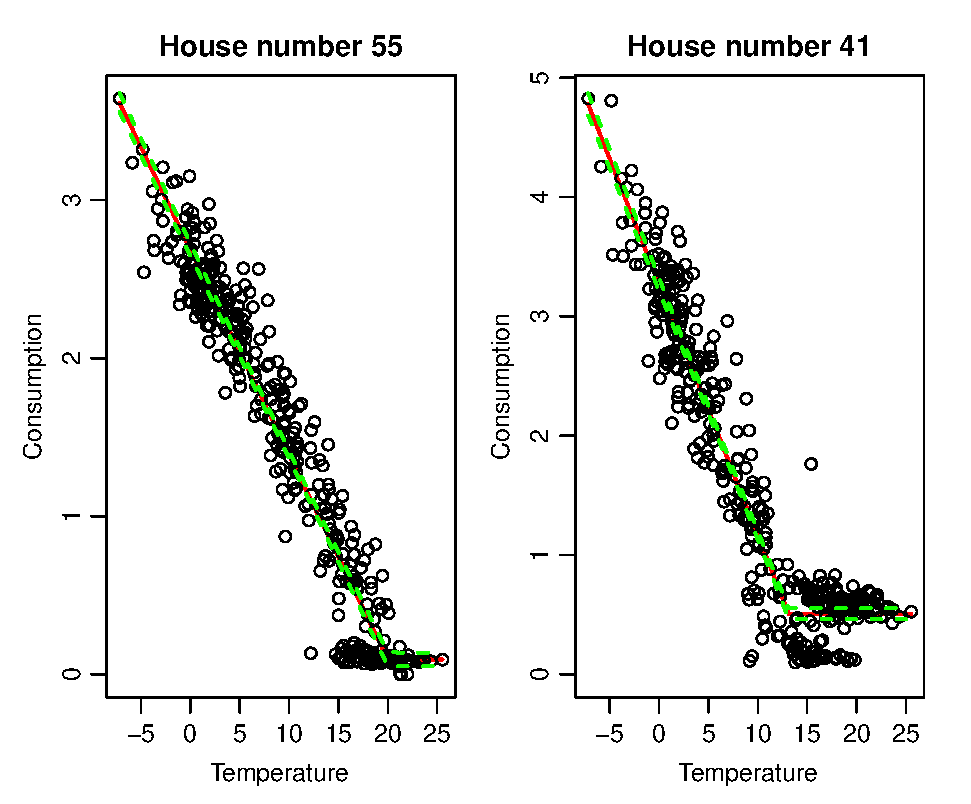
\includegraphics[width=\textwidth]{../../../figures/Consumption-PW.eps}
    \caption{Piece wise optimization of the consumption. The red line is the regression line and the green line is the confidence interval.}
    \label{fig: Consumption-PW}
\end{figure}
\subsection{Segmentation by investigation slopes}

\subsection{Segmentation by significant deviations}

%\subsection{Bestemmelse af temperatur breakpoint:}
%\begin{itemize}
%    \item Vi kigger på de huse der har mindst et års data (så vi er sikker på at hele sommeren er med)
%    \item Vi antager at dagene med over 20 grader udenfor, der er der slukket for varmen, og der er dermed kun varmvandsforbruget med, som vi antager er hvid støj.
%    \item For hver grad under 20 ser vi hvor mange procent af consumptionen der ligger indenfor +-2 standardafvigelser fra 20+ sættet.
%    \item Den første grad hvor mere end 20\% af datapunkterne ligger indenfor intervallet gemmes som det hus' alpha.
%    \item vi tager til sidst 15\% "percentile" af alphaerne, og skærer alt data fra vores datasæt som er over 12 grader.
%\end{itemize}

\section{BBR data}

\begin{itemize}
    \item Vi tager gennemsnittet af consumption over alle dage under 12 grader for hvert hus.
    \item Dette bliver divideret med det samlede boligareal.
    \item Når dette gøres ses 1 tydelig outlier, der tilhører en lejlighed på 61 $m^2$ bygget i 1920.
    \item Når vi plotter gennemsnitsconsumption med det seneste ombygningsår, ser vi en tendens af, at jo senere huset er blevet bygget om, jo mindre er varmeforbruget for huset.
\end{itemize}    

\section{Multicollinearity}
Multicollinearity occurs when two or more explanatory variables are highly correlated. In linear regression, multicollinearity 



\noindent The complete data set used for modeling in chapter 4 can be seen in table \ref{tab: modeldata} 
\begin{table}[H]
    \centering
    \begin{tabular}{ll}
     \hline
     \textbf{Variable} & \textbf{Description} \\
    \hline
    \hline
    Date  &  End time and date for measurements. Hourly values.\\
    Temperature  &  Temperature outside in Degrees/C. \\
    WindSpeed  &  \\
    WindDirection  &  \\
    SunHour  &  \\
    Condition  & \\
    UltravioletIndex  &   \\
    MeanSeaLevelPressure  & \\
    PrecipitationProbability & \\
    Observation & \\
    Consumption & CoolingDegree times Volume from House data \\
    Holiday & \\
    \hline
    \end{tabular}
    \caption{Attributes used for modelling.}
    \label{tab: modeldata}
\end{table}   